\section{Gestão dos Riscos}
\label{levantamentoRiscos}

A Gestão de Risco é um processo de identificação, análise, avaliação, tratamento e monitoramento de um evento que pode atrasar uma entrega de um produto ou serviço. A ISO 31000 define como atividades coordenadas para dirigir e controlar uma organização no que se refere a riscos \cite{purdy2010iso}.
Neste projeto, a gestão de risco é feita utilizando práticas da metodologia ágil, onde os riscos Técnicos, Externos, Organizacionais e relacionados ao Gerenciamento são levantados e acompanhados a cada  \textit{Sprint}, a fim de reduzir a probabilidade do risco acontecer \cite{cohn_RiskBurndown_blog2010}.

Para isso, criamos um \textit{burndown} de Riscos que auxilia no acompanhamento dos riscos por \textit{Sprints}, verificando a probabilidade e o impacto do risco, a fim de reagir a tempo. Esse modelo de gestão de riscos baseia-se em uma métrica subjetiva, pois o próprio time define o impacto e a probabilidade do risco acontecer. 

O processo de identificação, análise, avaliação, tratamento e monitoramento de um evento (interno ou externo) que pode ser um risco para o projeto é feito em todas as {\em sprints}, sendo que cada {\em sprint} cobre o período de uma semana. Primeiramente, é feito um levantamento de todos os $N$ eventos potenciais de risco ao projeto. Cada item desse levantamento é avaliado periodicamente, levando-se em conta dois fatores: a chance de o risco ocorrer $P$ e o impacto disso $I$. No nosso caso, ambos fatores ($P$ e $I$) são anotados usando valores que vão de 0 a 5, indicando as seguintes avaliações qualitativas de probabilidade de cada evento ocorrer: nenhum; raro; improvável; pouco provável; 
muito provável; quase certo. Os cálculos e o acompanhamento dos riscos estão disponíveis na planilha de Riscos por meio do link a seguir: \href{https://docs.google.com/spreadsheets/d/1TQ4I9uqX-XxH3AdRi01n4jIX4YpIWYOHws1GxpdqUF0/edit?usp=sharing}{Planilha de Acompanhamento dos Riscos}.

\begin{figure}[ht]
  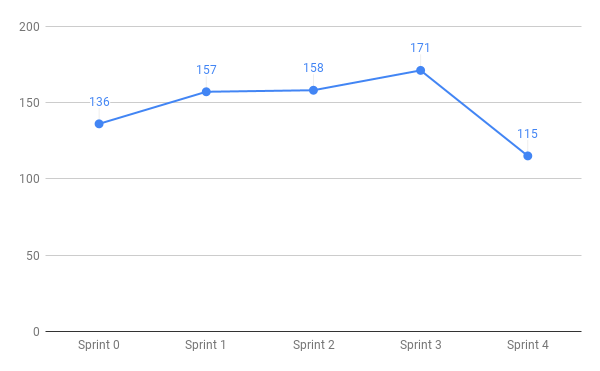
\includegraphics[scale=0.75]{figuras/burndownrisco.png}
  \caption{\textit{Risk Burndown} geral: multiplição da  probabilidade do evento do risco pelo impacto do evento no desenvolvimento do projeto, durante a Release 1.} 
  \label{fig:riscogeral}
\end{figure}

O fator {\em Risk Burndown} (eixo Y no gráfico da figura \ref{fig:riscogeral}) é calculado multiplicando-se esses dois fatores e somando os resultados para todos os $N$ eventos avaliados.
Até o momento, foram identificados $N=17$ fatores de risco, ou seja, o maior valor possível para o fator {\em risk burndown} deste projeto atualmente seria de $N \times P \times I = 17 \times 5 \times 5 = 425$, num cenário de caos absoluto.
Porém, não é de se esperar que todos os fatores tenham impacto máximo e máxima probabilidade de acontecer ao mesmo tempo, por isso o gráfico da figura \ref{fig:riscogeral} mostra o eixo Y indo somente até 200.

Durante a análise da probabilidade, são definidas ações para mitigar o risco. Desde o início do projeto, os principais riscos foram ligados à cultura e organização das atividades, definição do escopo para atender às necessidades do cliente e à pandemia. É possível notar o crescimento de risco do projeto na {\em Sprint} 3, devido a identificação de novos riscos, mas é possível notar na Imagem \ref{fig:riscogeral} que os riscos estão diminuindo constantemente.